\documentclass[12pt]{article}

 %%%%%%%%%% LOADING PACKAGES %%%%%%%%%% 
\usepackage{amsmath, amssymb, amsfonts, bm, mathtools} % math packages
\usepackage[table]{xcolor}
\usepackage{physics}
\usepackage{graphicx}
\usepackage{parskip}
\usepackage{fancyhdr}
\usepackage{vmargin}
\usepackage{tcolorbox}
\usepackage{url}
\usepackage[utf8x]{inputenc}
\usepackage{hyperref} % to click and go to pointed place in the document
\usepackage{cancel} % for easy cancellations
\usepackage{minted} % for highlighting code
\usepackage{comment} % for multi-line commenting

 %%%%%%%%%% SET DEFAULTS %%%%%%%%%% 
\newcommand{\smallspace}{\hspace{0.5cm}}
\setcounter{secnumdepth}{0} % for avoiding the numbering
\newenvironment{sfemph}{\begin{sffamily}\begin{emph}}{\end{sffamily}\end{emph}}
 % the text inside the exercise setup will be emphasized
 % Set defaults for minted
\setminted{frame=lines,
framesep=2mm,
baselinestretch=1.2,
bgcolor=,
fontsize=\footnotesize,
linenos
}

 %%%%%%%%%% INSERT YOUR DATA HERE %%%%%%%%%% 
\title{Stock Price Prediction with Sentiment Analysis}						
\author{Federico Berto}			 				
\date{\today}											
\newcommand{\professor}{Woo Chang Kim}
\newcommand{\studentid}{20204817}
\newcommand{\coursename}{Introduction to Financial Engineering}
\newcommand{\courseid}{IE471}
\newcommand{\firstuniversityline}{Korea Advanced Institute of Science} % first line of university name
\newcommand{\seconduniversityline}{and Technology} % split the title for better compatibility. You may modify this part

 %%%%%%%%%% TITLE PAGE SETUP %%%%%%%%%% 
\setmarginsrb{3 cm}{2.5 cm}{3 cm}{2.5 cm}{1 cm}{1.5 cm}{1 cm}{1.5 cm}
\makeatletter
\let\thetitle\@title
\let\theauthor\@author
\let\thedate\@date
\makeatother
\pagestyle{fancy}
\fancyhf{}
\renewcommand{\headrulewidth}{0.4pt}
\rhead{\theauthor}
\lhead{AI Project 1}
\chead{\raisebox{-1ex}{
\includegraphics[width = 3cm]{images/university_secondary_logo.png}}}
\cfoot{Page \thepage}

 %%%%%%%%%% MAIN DOCUMENT %%%%%%%%%% 
\begin{document}

 %%%%%%%%%% TITLE PAGE SETUP %%%%%%%%%% 
\begin{titlepage}
	\centering
    \textsc{\LARGE  \firstuniversityline \\ \smallskip \seconduniversityline}\\[1 cm]	% university Name
    
\includegraphics[scale = 0.18]{images/university_main_logo.png}\\[1.5 cm]	% university Logo
    
	\textsc{\Large \coursename}\\[0.5 cm]
	\rule{\linewidth}{0.2 mm} \\[0.4 cm]
	{ \huge \bfseries {\thetitle}}\\
	\rule{\linewidth}{0.2 mm} \\[1.5 cm]
	
	\begin{minipage}{0.5\textwidth}
		\begin{flushleft} \large
			\emph{Professor:}\\
		    \professor \\ [0.5cm]
            \emph{Course ID:}\\
            \courseid
			\end{flushleft}
			\end{minipage}~
			\begin{minipage}{0.4\textwidth}
			\begin{flushright} \large
			\emph{Student:} \\
			\theauthor \\[0.5cm]
			\emph{ID number:}\\
			\studentid \\
		\end{flushright}
	\end{minipage}\\[2 cm]
	
\end{titlepage}

 %%%%%%%%%% TABLE OF CONTENTS %%%%%%%%%% 
%% Uncomment this part
% \tableofcontents
% \incl
% \pagebreak


 %%%%%%%%%% MAIN TEXT %%%%%%%%%% 
\section{Introduction}

The goal of this report is to describe the experimental process and result for predicting stock price with the help of \textit{sentiment analysis} based on Twitter data. In particular, in the first experiment we will predict Tesla, Inc adjusted closing stock price in the last quarter of 2020 \footnote{Source: \href{https://finance.yahoo.com/quote/TSLA/}{Yahoo Finance}} using data from the first three quarters.\\
Let us briefly introduce the models we will use in the code.

\subsection{Recurrent Neural Networks}
\label{sec:rnn}
Recurrent Neural Networks (RNN) \cite{zaremba2014recurrent} are capable of dealing with sequences of data. As Figure \ref{fig:rnn} \footnote{Source: \href{https://kvitajakub.github.io/2016/04/14/rnn-diagrams/}{Github}}  shows, they form an unrolled, sequential undirected graph in which input data are fed sequentially.
\begin{figure}[h!]
    \centering
    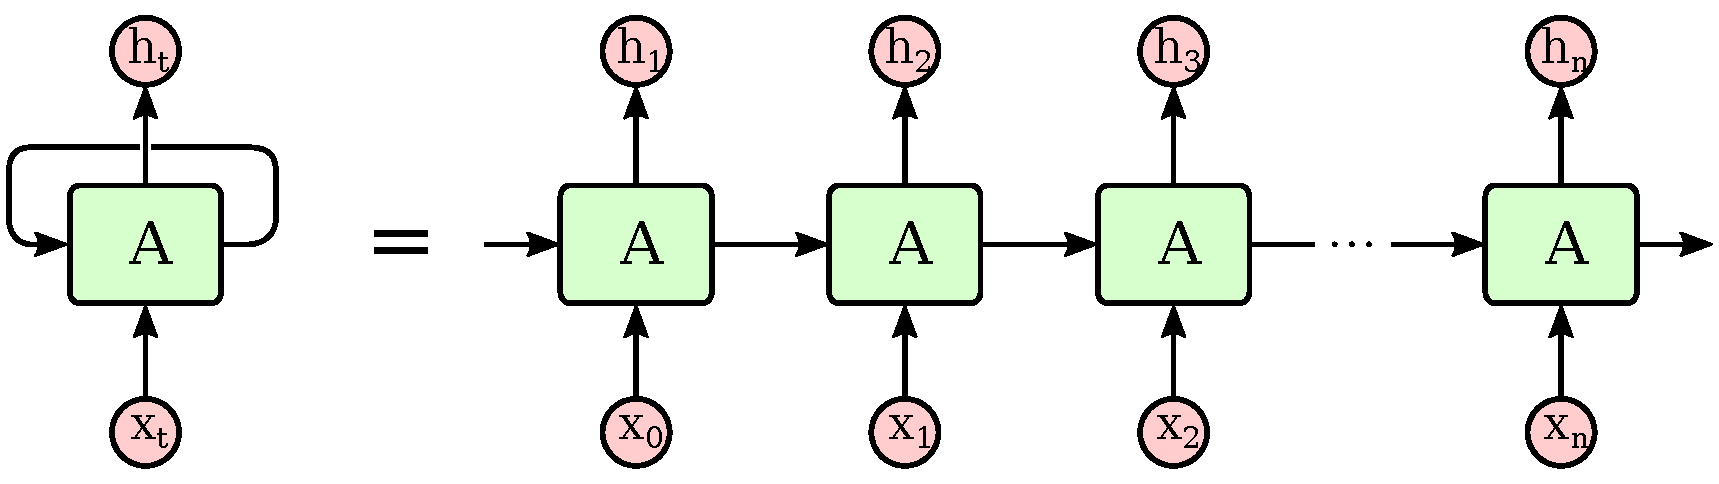
\includegraphics[width=0.7\linewidth]{images/rnn.pdf}
    \caption{Recurrent Neural Network (RNN) base model}
    \label{fig:rnn}
\end{figure}
The vanilla implementation's most notable problem is the so-called \textit{vanishing gradients} problem, in which long time series cannot be dealt with due the parameter updates using gradients; due to the sequential nature of RNNs, the further inputs in the time series are subject to more activation functions, causing updates to be almost independent from them.\\
For this reason, more advanced versions of Recurrent Neural Networks i.e GRU and LSTM have been created. Nonetheless, the simplicity of RNNs makes them suitable for shorter and less complex time series, since they are faster and also less prone to overfitting due to less parameters.

\subsection{Gated Recurrent Units}
\label{sec:gru}
Gated Recurrent Units (GRU) \cite{cho2014learning} were proposed as an RNN variant in 2014: they are similar to LSTMs without an output gate and has fewer parameters. Figure \ref{fig:gru} \footnote{Source: \href{https://en.wikipedia.org/wiki/Gated_recurrent_unit}{Wikimedia}} shows an overview of the architecture.
\begin{figure}[h!]
    \centering
    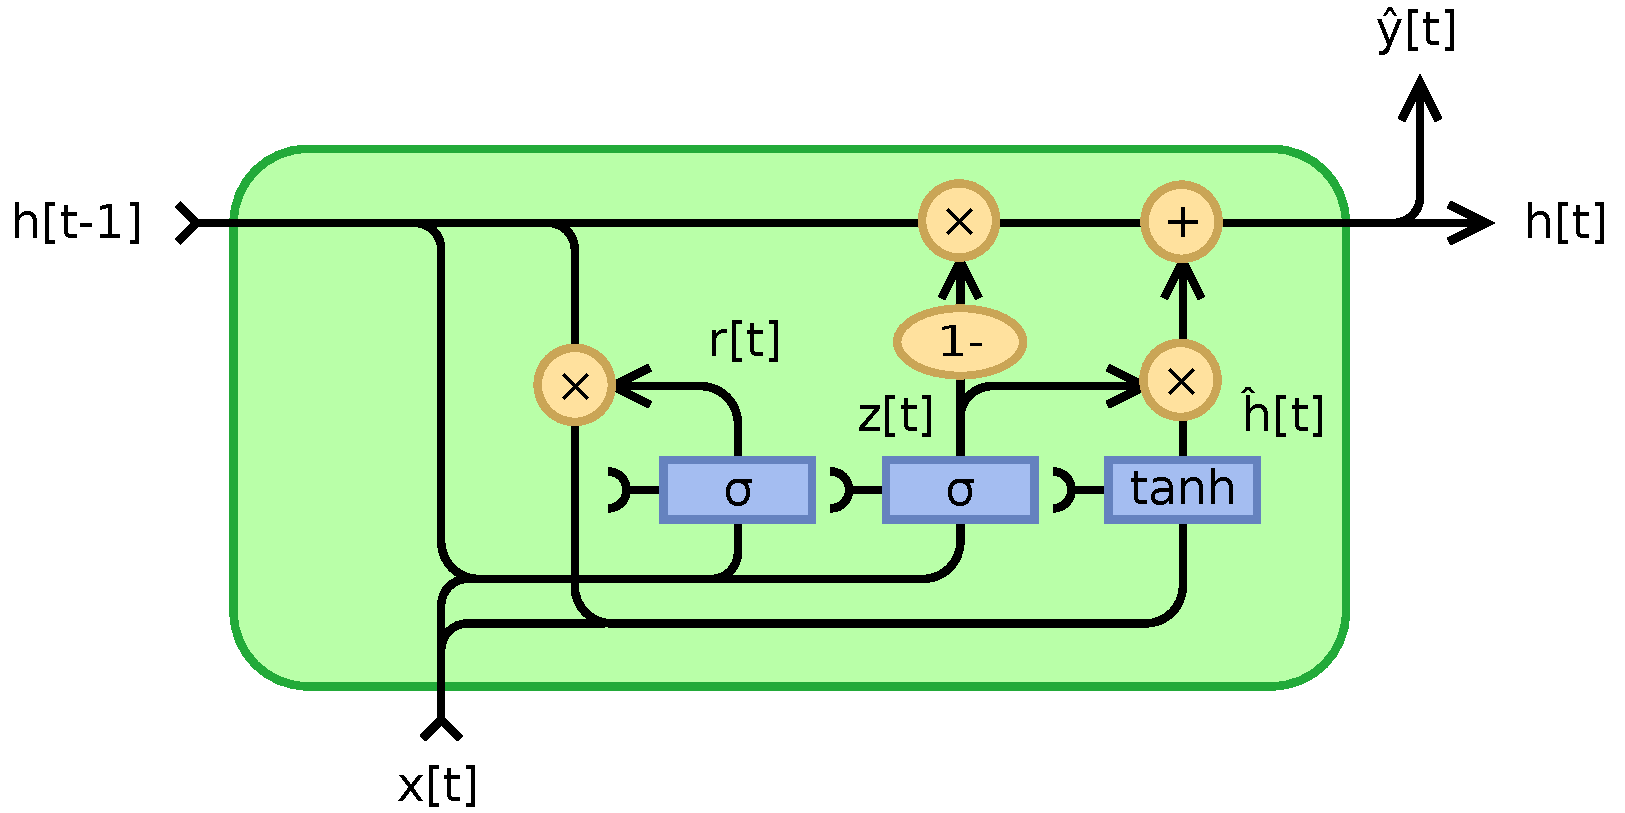
\includegraphics[width=0.7\linewidth]{images/Gated_Recurrent_Unit,_base_type.pdf}
    \caption{Gated Recurrent Unit (GRU) base model}
    \label{fig:gru}
\end{figure}
Having fewer parameters than LSTM \ref{sec:lstm}, GRUs have been shown to perform better on certain dataset and have better generalization capabilities with fewer data.

\subsection{Long Short-Term Memory}
\label{sec:lstm}
The prediction model is based on the Long Short-Term Memory (LSTM) \cite{hochreiter1997long} module in Figure \ref{fig:LSTM}\footnote{Source: \href{https://commons.wikimedia.org/wiki/File:LSTM_cell.svg}{Wikimedia}}, which is able to store past information of the data and is thus suitable for time series prediction.

\begin{figure}[h!]
    \centering
    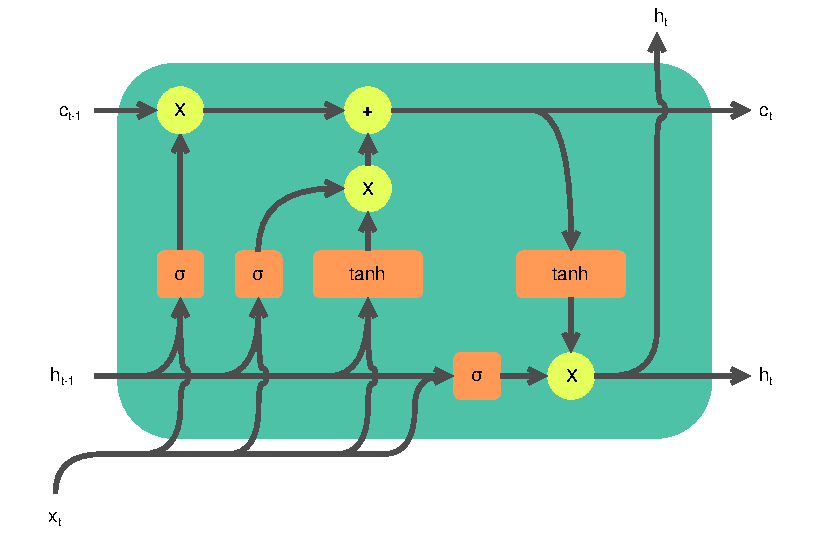
\includegraphics[width=0.7\textwidth]{images/LSTM_cell.pdf}
    \caption{LSTM cell}
    \label{fig:LSTM}
\end{figure}

Further details into the PyTorch \cite{pytorch} implementation can be found in the code, also available on the following \href{https://github.com/Juju-botu/financial-engineering-ai}{Github repository}.\footnote{Link: \href{https://github.com/Juju-botu/financial-engineering-ai}{\tt{https://github.com/Juju-botu/financial-engineering-ai}}.}

\subsection{Sentiment Analysis with Twitter Data}
We use sentiment analysis \cite{Mittal2011StockPU} in order to get better predictions on the original dataset: our goal is to capture public \textit{trends} via Twitter data scraping. 

\begin{figure}[h!]
    \centering
    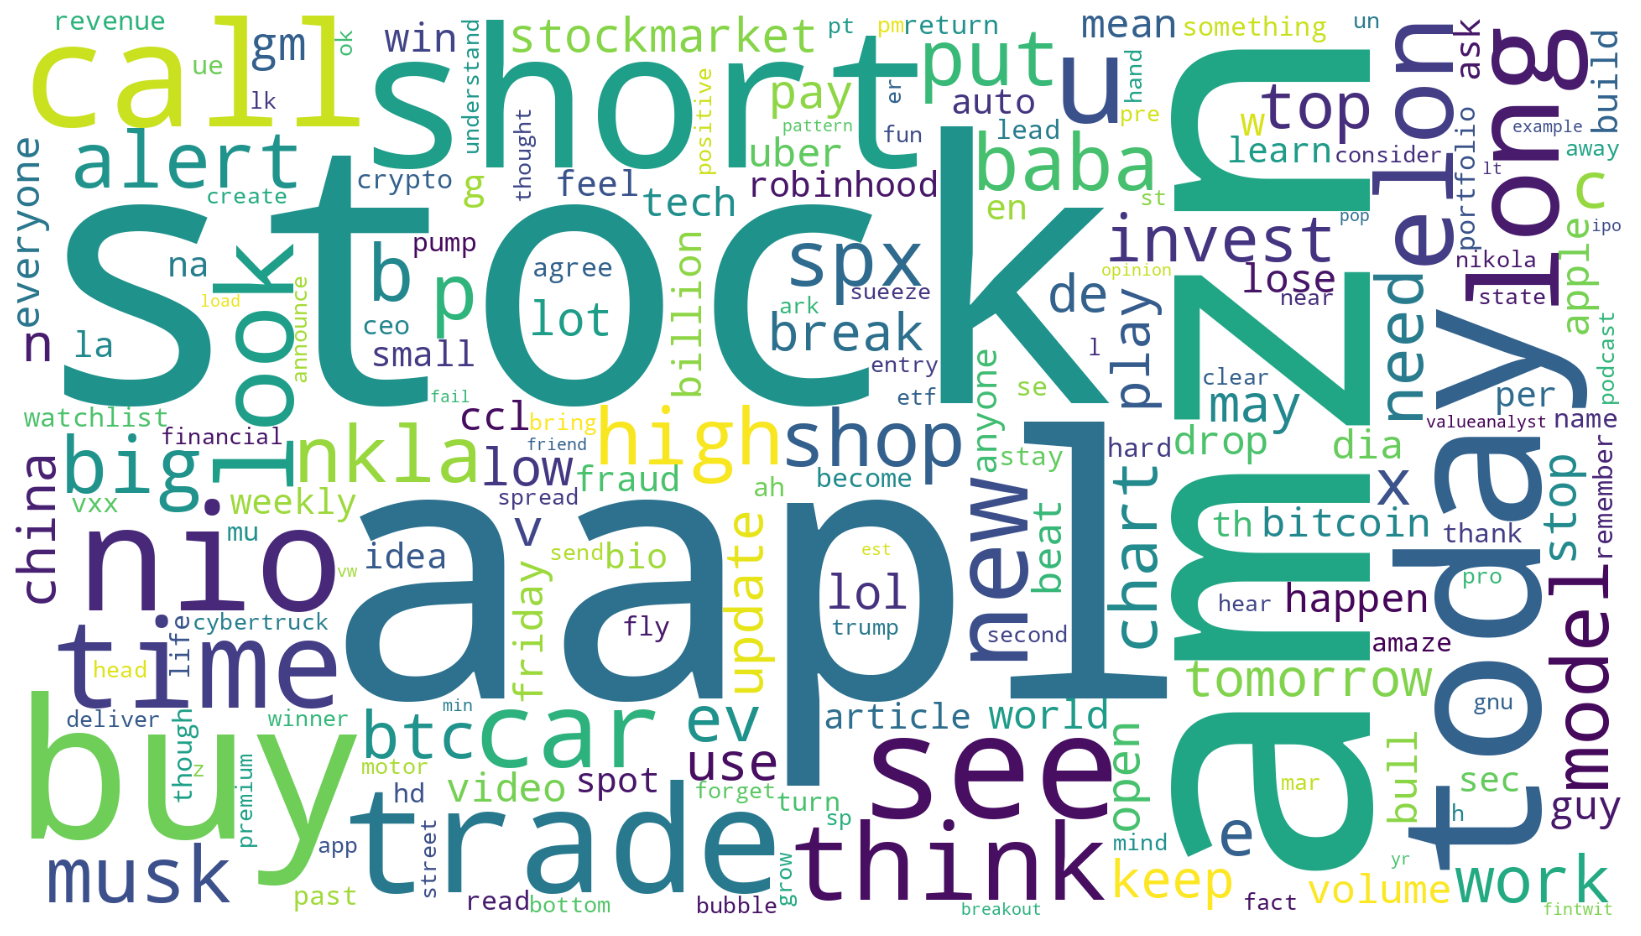
\includegraphics[width=0.7\textwidth]{images/wordcloud_simple.pdf}
    \caption{Word cloud of most popular words related to Tesla on Twitter}
    \label{fig:tesla_wordcloud}
\end{figure}

We use natural language processing with TextBlob \footnote{Source: \href{https://github.com/sloria/textblob}{Github}} to capture these trends and convert them to usable numbers.

\section{Experiments}

\subsection{Predicting Tesla's Stock Price}
In this section we provide the required data for the report.

\paragraph{1.} Mean Squared Error values for the whole dataset, training data and test data without sentiment analysis:

\begin{center}
\rowcolors{2}{gray!25}{white}     
    \begin{tabular}{l rl}
    \rowcolor{gray!50}
         &  \textbf{MSE}\\
         \hline
         \text{Whole dataset} & 1312.9493\\
         \text{Training Data} & 39.4943\\
         \text{Test Data} & 4995.5659\\
    \end{tabular}
\end{center}

\paragraph{2.} Word cloud image of cleaned tweets: Figure \ref{fig:tesla_wordcloud_logo}.

\begin{figure}[h!]
    \centering
    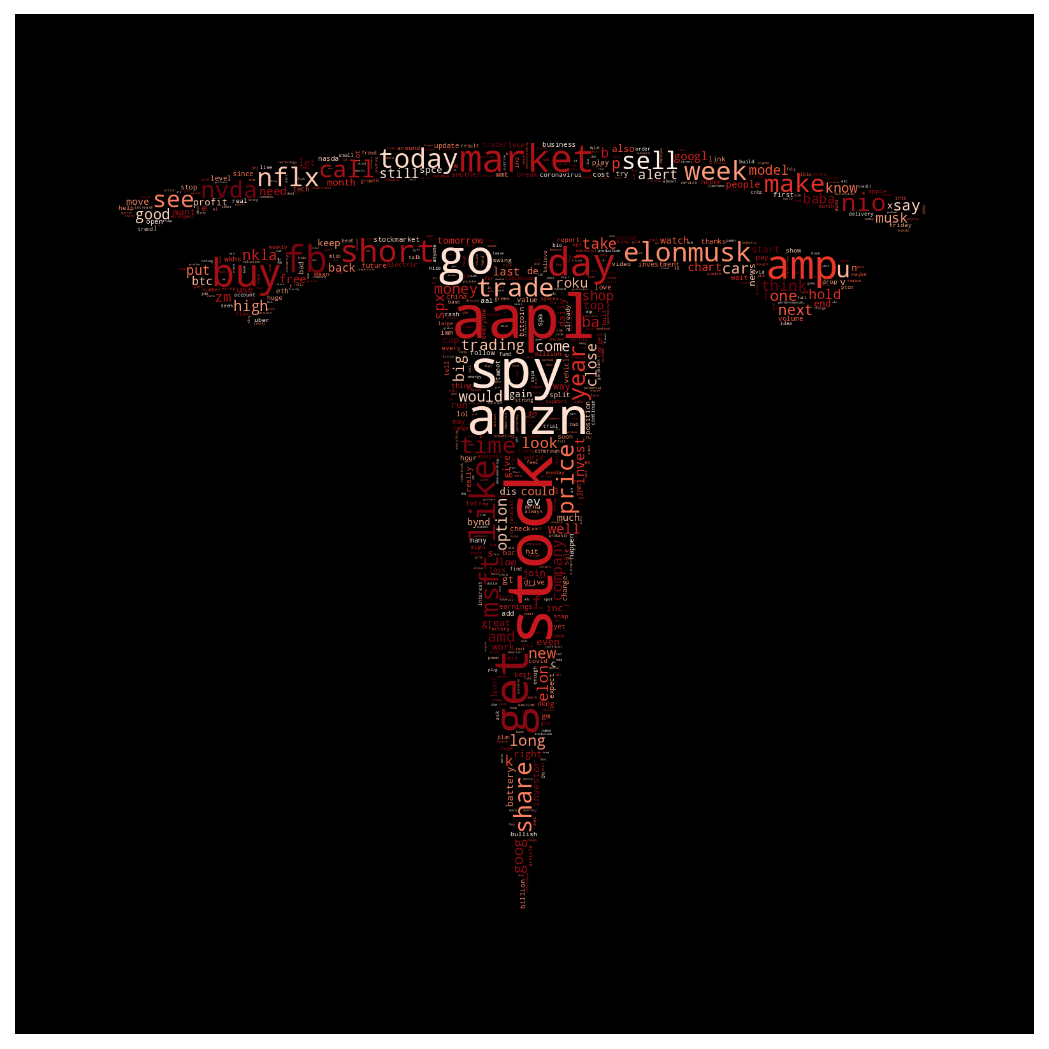
\includegraphics[width=0.9\textwidth]{images/wordcloud.pdf}
    \caption{Word cloud of most popular words related to Tesla on Twitter}
    \label{fig:tesla_wordcloud_logo}
\end{figure}

\paragraph{3.} Bar chart of 20 most frequent words of cleaned tweets: Figure \ref{fig:bar_chart}.

\begin{figure}[h!]
    \centering
    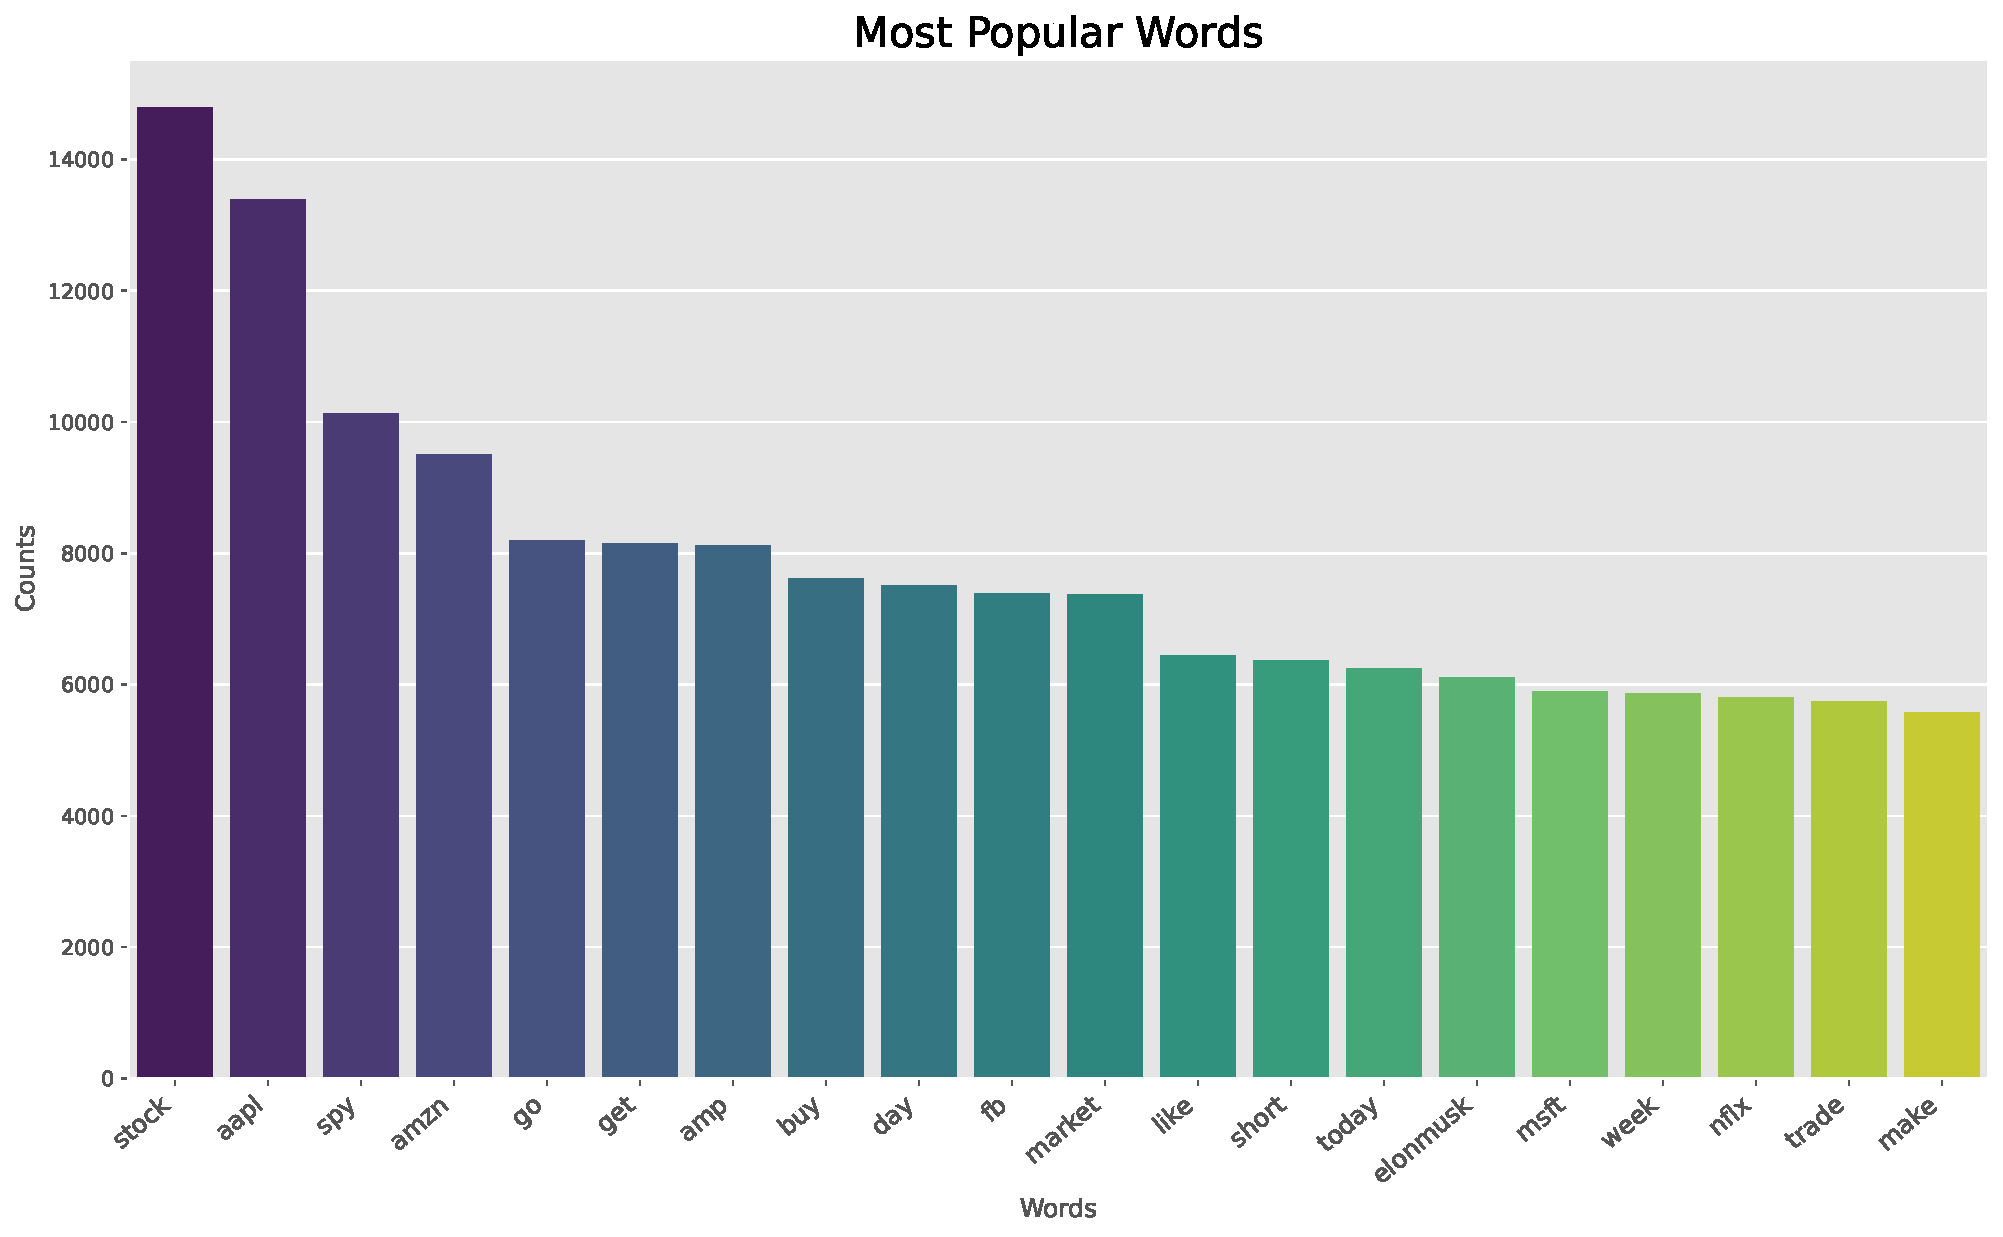
\includegraphics[width=0.7\textwidth]{images/popular_words.pdf}
    \caption{Bar chart most popular words related to Tesla on Twitter}
    \label{fig:bar_chart}
\end{figure}

\paragraph{4.} ID and sentiment scores of first five cleaned tweets:
\begin{center}
\rowcolors{2}{gray!25}{white}     
    \begin{tabular}{l rl}
    \rowcolor{gray!50}
         \textbf{ID} &  \textbf{Sentiment Score}\\
         \hline
         1212450794705969152 & 0.15\\
         1212450579634626560 & -0.20\\
         1212450337543602177 & 0.20\\
         1212450309131227141 & 0.00\\
         1212449703318753280 & 0.75\\
    \end{tabular}
\end{center}

\paragraph{5.} Average sentiment score before removing 0 and after, January 1$^{st}$ to 5$^{th}$:
\begin{center}
\rowcolors{2}{gray!25}{white}     
    \begin{tabular}{l cl rl}
    \rowcolor{gray!50}
        \bf{Date} & \bf{Sentiment} & \bf{Sentiment Final}\\
        \hline
        2020-01-01 &    0.099938&	0.154961\\
        2020-01-02 &	0.111398&	0.161528\\
        2020-01-03 &	0.073760&	0.128297\\
        2020-01-04 &	0.083606&	0.144796\\
        2020-01-05 &	0.086658&	0.132267\\
    \end{tabular}
\end{center}

\paragraph{6.}  Mean Squared Error values for the whole dataset, training data and test data \textit{with} sentiment analysis:
\begin{center}
\rowcolors{2}{gray!25}{white}     
    \begin{tabular}{l rl}
    \rowcolor{gray!50}
         &  \textbf{MSE}\\
         \hline
         \text{Whole dataset} & 669.5747\\
         \text{Training Data} & 42.2973\\
         \text{Test Data} & 2483.8538\\
    \end{tabular}
\end{center}

\paragraph{7. } \textit{Comparison of the results before and after sentiment analysis}: we compare in Figure \ref{fig:tesla_comparison_with_without} the results of LSTM with and without sentiment analysis.
\begin{figure}[h!]
    \centering
    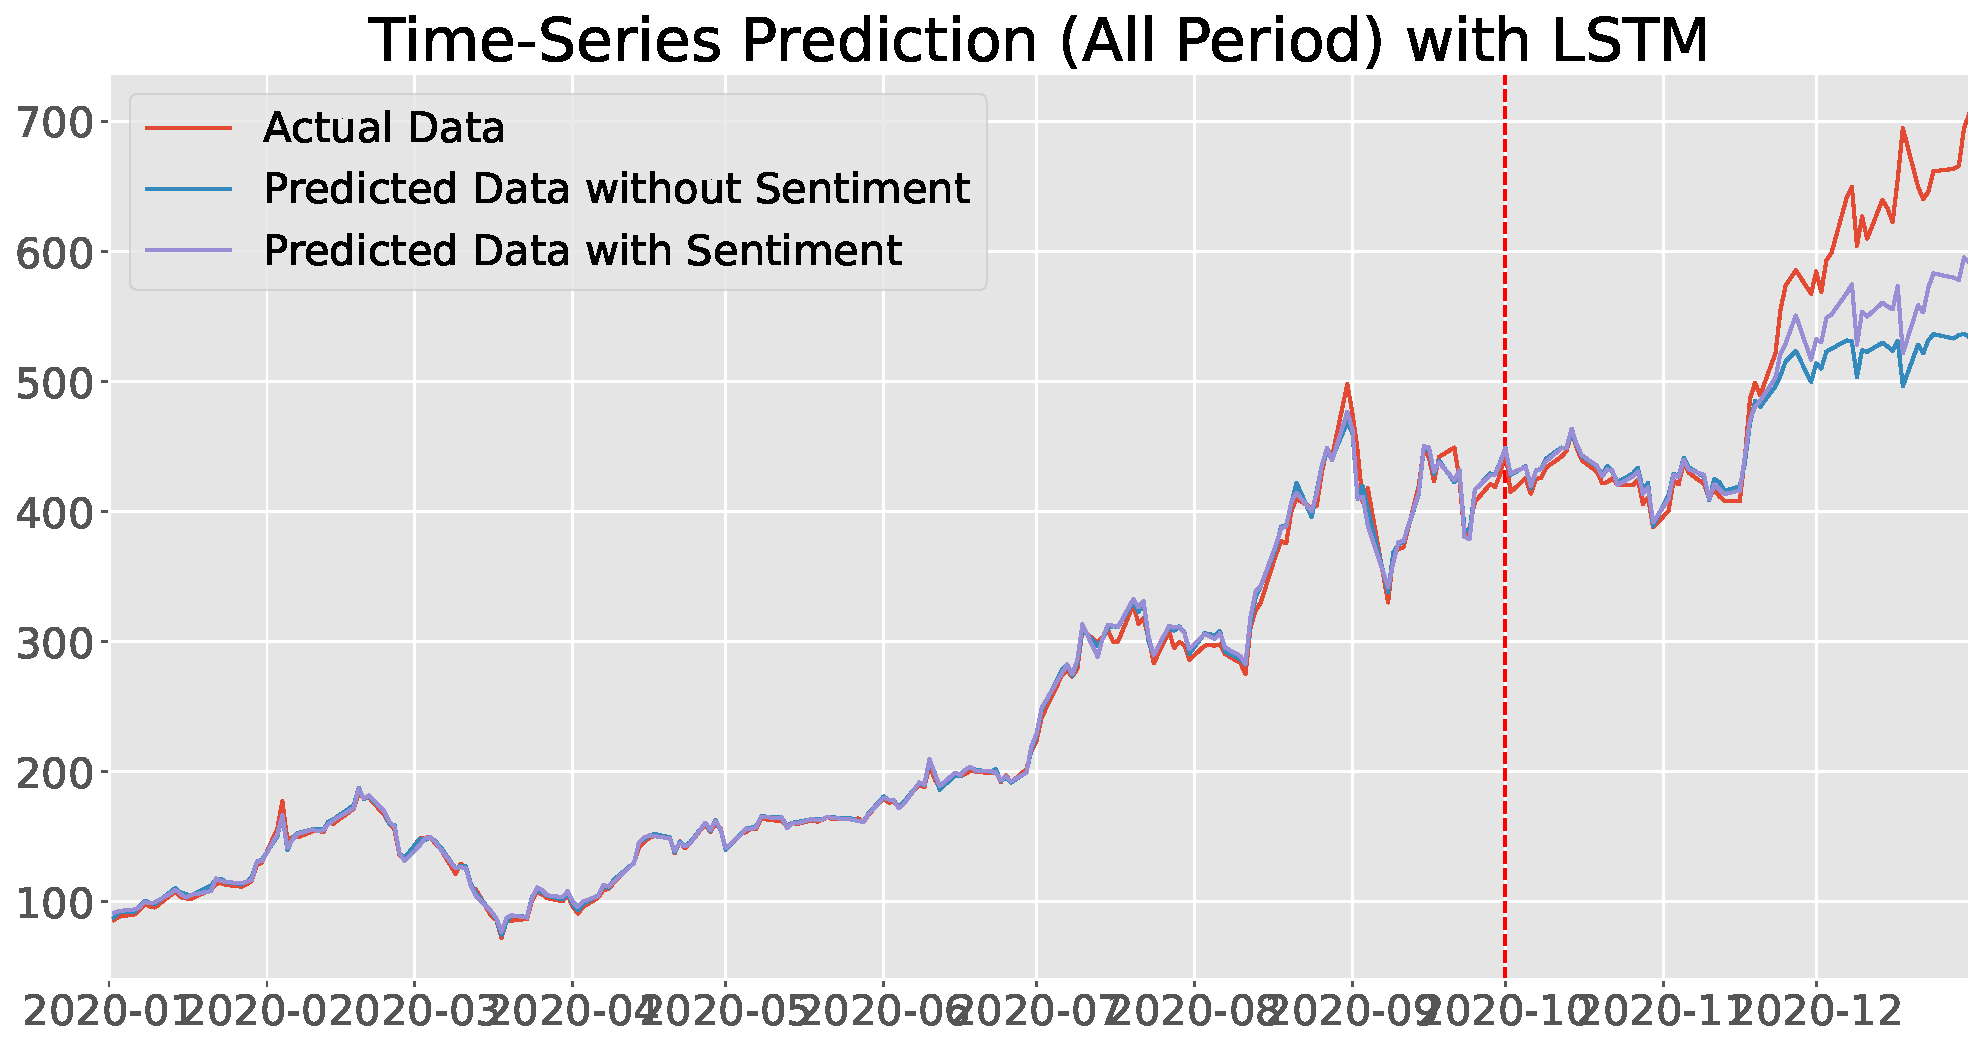
\includegraphics[width=0.8\textwidth]{images/lstm_with_without_sentiment_all.pdf}
    \caption{Comparison of LSTM's predictions without and with sentiment analysis}
    \label{fig:tesla_comparison_with_without}
\end{figure}

\begin{center}
\rowcolors{2}{gray!25}{white}     
    \begin{tabular}{l cl rl}
    \rowcolor{gray!50}
         & \textbf{MSE - Without Sentiment} & \textbf{MSE - With Sentiment}\\
         \text{Whole dataset} & 1312.9493 & 669.5747\\
         \text{Training Data} & 39.4943 & 42.2973\\
         \text{Test Data} & 4995.5659 & 2483.8538\\
    \end{tabular}
\end{center}
As we can see, sentiment analysis is able to help with predictions and was able to reduce by half the MSE in the testing region. However, it should be noted that due to the limited size of the dataset, the training results have a high variance; nonetheless, we noticed an improvement on the prediction cababilities of the network even across multiple experiments.

\section{Improving the Predictions}
In this section, we show how to improve the algorithm in three ways:
\begin{enumerate}
    \item Revising the codes with Pytorch Lightning
    \item Using a different AI algorithm, namely Recurrent Neural Networks (RNN) \ref{sec:rnn} and Gated Recurrent Unit (GRU) \ref{sec:gru}
    \item Improving the MSE error results
\end{enumerate}

\subsection{Using Pytorch Lightning}
We revise the code by using Pytorch Lightning \cite{falcon2019pytorch}: this PyTorch framework provides a high-level interface by which it is easier to control architectures, results, logging and more. 
More importantly, it makes the process of moving models to GPU, Tensor Processing Units (TPUs) and even multiple GPUs and TPUs easier while having a negligible overhead. This open-source library is actively maintained by a community highly focused on efficiency and code readability. We refactor the code to be used with Pytorch Lightning.

\subsection{Results Comparison}
We show in Figure \ref{fig:comparison} a comparison of the algorithms run with the same parameters with Pytorch Lightning.
\begin{figure}[h!]
    \centering
    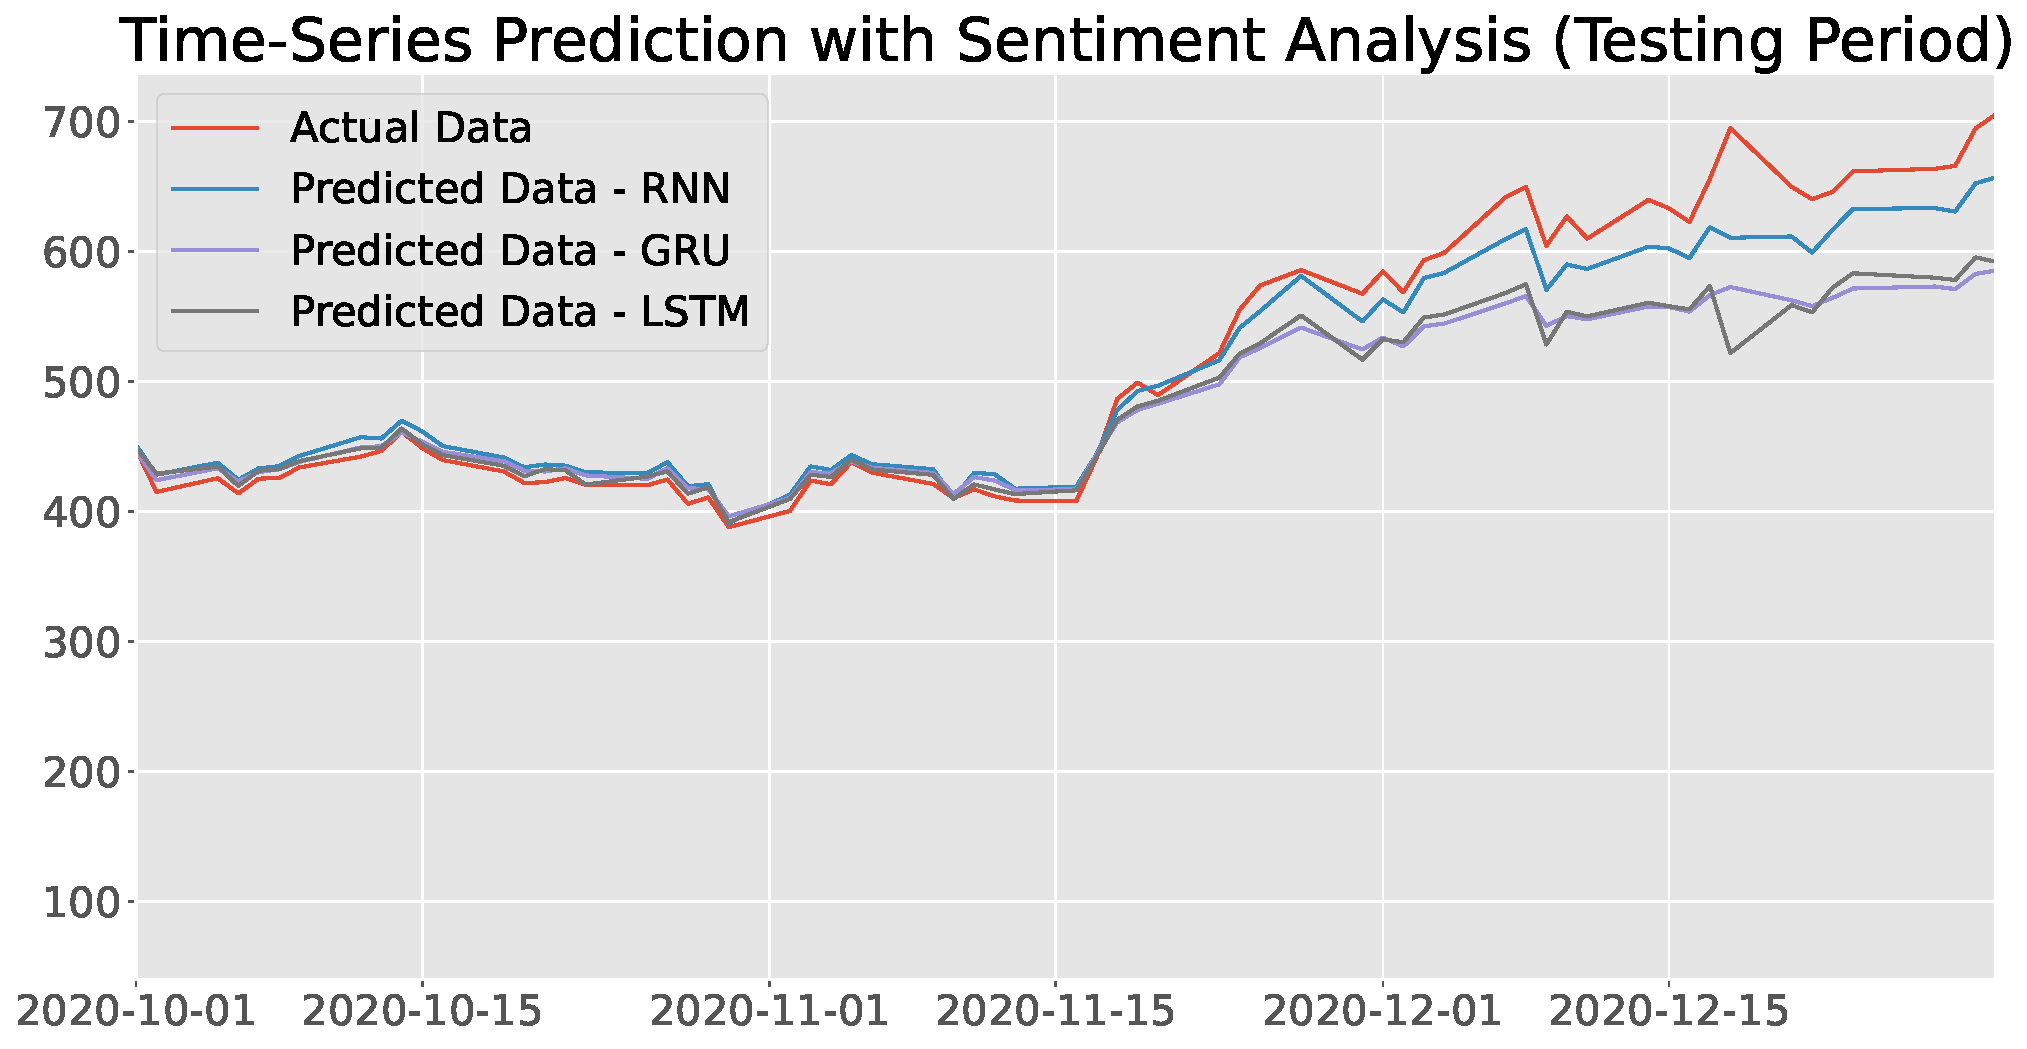
\includegraphics[width=0.8\textwidth]{images/comparison.pdf}
    \caption{Comparison of different algorithms on Tesla's stock price prediction with sentiment analysis}
    \label{fig:comparison}
\end{figure}
We also report the MSE table for the different approaches:
\begin{center}
\rowcolors{1}{gray!25}{white}     
    \begin{tabular}{l cl cl rl}
    \rowcolor{gray!70}
    \multicolumn{4}{c}{\textbf{Mean Squared Error}}\\
    \hline
    \rowcolor{gray!50}
         & \textbf{RNN} & \textbf{GRU} & \textbf{LSTM}\\
         \text{Whole Dataset} & \textbf{156.5683} & 657.3547 & 669.5747\\
         \text{Training Data} & 29.5203 & \textbf{26.7311} & 42.2973\\
         \text{Test Data} & \textbf{524.0301} & 2481.3120  & 2483.8538 \\
    \end{tabular}
\end{center}
The results show that, while GRU and LSTM performed similarly on the training data, RNN was able to outperform them on the test set although it has lower complexity. One reason for this behavior could be that, since the test data ranges with previously unseen values, RNN is able to \textit{extrapolate} better and is less prone to overfitting on this particular dataset. Moreover, since we chose the sequence of data as 5, the vanishing gradients problem was not encountered.\\
This experiment demonstrates that on certain, simple enough datasets less advanced models such as RNN can be useful and even outperform more complicated ones.

\section{Predicting Nvidia's Stock price}
As an extension for the above experiments, we also predict Nvidia Stock Prices with the same time span of the previous experiments.\\


In order to do so, we first built a \textit{data scrapper} based on $\tt twint$ \footnote{Source: \href{https://github.com/twintproject/twint}{Github}} and extract data from Twitter. 

\begin{figure}[h!]
    \centering
    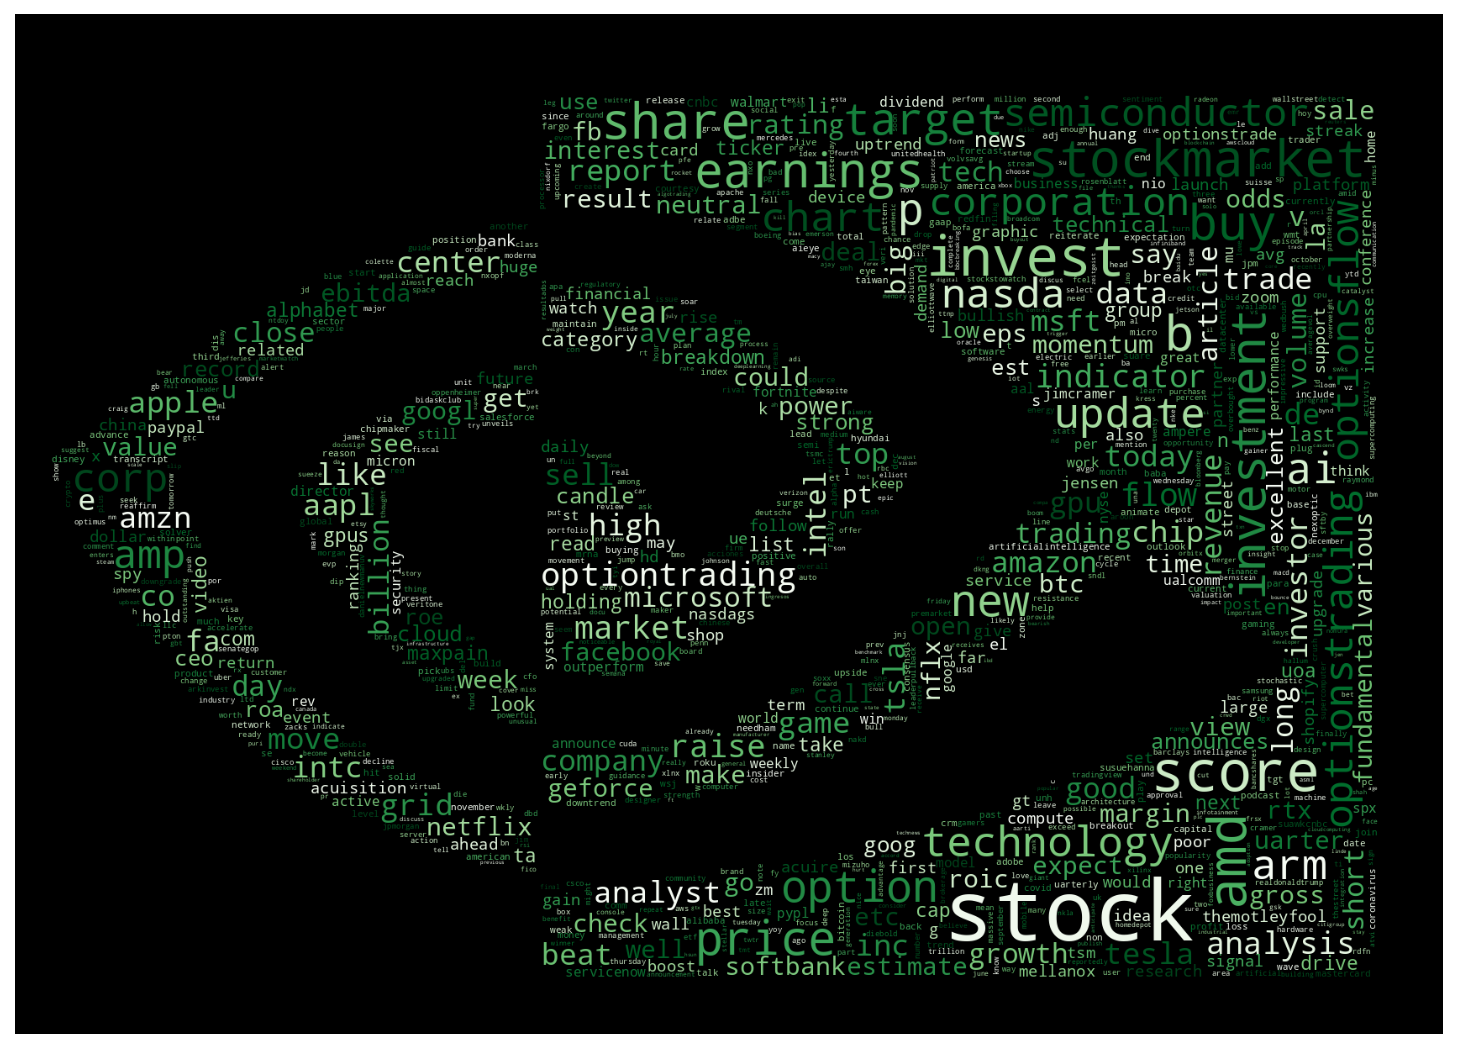
\includegraphics[width=0.9\textwidth]{images/wordcloud_nvidia.pdf}
    \caption{Word cloud of most popular words related to Nvidia on Twitter}
    \label{fig:nvidia_wordcloud}
\end{figure}

After using TextBlob for the Sentiment Analysis, we feed the data to our model. Figure \ref{fig:comparison_nvidia} shows the result graphically.
\begin{figure}[h!]
    \centering
    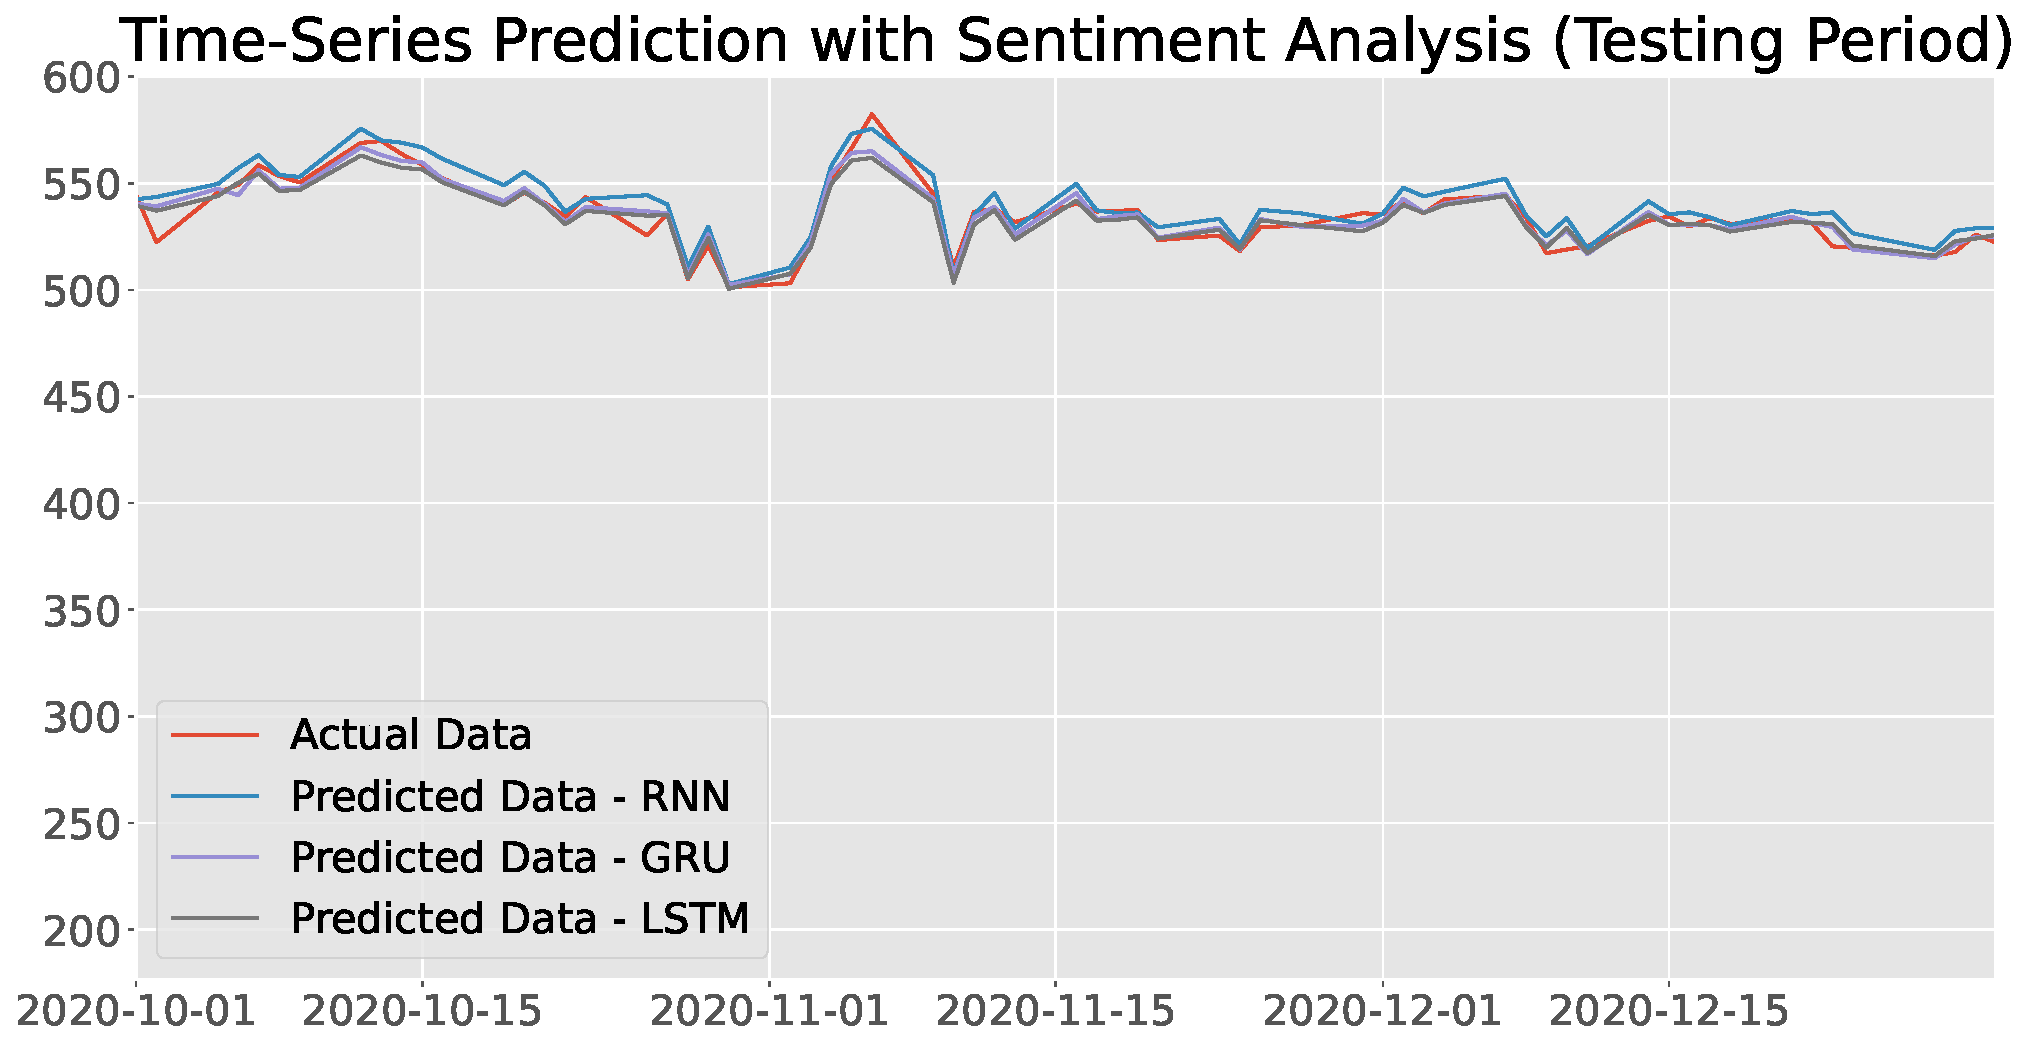
\includegraphics[width=0.9\textwidth]{images/nvidia_comparison.pdf}
    \caption{Comparison of different algorithms on Nvidia's stock price prediction with sentiment analysis}
    \label{fig:comparison_nvidia}
\end{figure}

We also report the MSE table for the different approaches:
\begin{center}
\rowcolors{1}{gray!25}{white}     
    \begin{tabular}{l cl cl rl}
    \rowcolor{gray!70}
    \multicolumn{4}{c}{\textbf{Mean Squared Error}}\\
    \hline
    \rowcolor{gray!50}
         & \textbf{RNN} & \textbf{GRU} & \textbf{LSTM}\\
         \text{Whole Dataset} & 39.2606 &  \textbf{27.7972} & 28.0963\\
         \text{Training Data} & 35.3114 & 29.8236 & \textbf{28.0955}\\
         \text{Test Data} & 50.6829 &  \textbf{21.9361} & 28.0985 \\
    \end{tabular}
\end{center}
From this experiment, we obtain a similar result of our previous report on stock market prediction without sentiment analysis: GRU seems to perform better than LSTM, possibily due to its ability to deal with overfitting. Given that the predicted data were in the same range of values as the training data, the RNN's advantage in extrapolation was overcome by the more encompassing representation of more advanced models. \\
We noticed in both experiments that LSTM does not perform equally well as its less complex counterparts on smaller datasets, in which it is more prone to overfitting the training data.

 %%%%%%%%%% BIBLIOGRAPHY %%%%%%%%%% 
\bibliographystyle{plain}
\bibliography{ref}

\end{document}